\chapter{Auswertung und Diskussion} \label{ch:crispDm_3}

Dieses Kapitel evaluiert einerseits die \nameref{ch:crispDm_1} und das \nameref{ch:crispDm_2}.

In der Diskussion werden zunächst die Entscheidungen und Prozesse in dieser Arbeit kritisch hinterfragt. Weiterhin weist der Abschnitt auf Schwachstellen und Biases hin, die sich in \autoref{ch:crispDm_2} ergeben haben.

\section{Kritische Betrachtung} \label{subsec:discussion}

Wie in \autoref{sec:representationForms} erklärt, bieten kontextunabhängige Methoden nur begrenzte Möglichkeiten, semantische Zusammenhänge abzubilden. Somit stellt sich die Frage, inwiefern Modelle, die mit \ac{BoW}, \ac{TF-IDF} und \ac{GloVe} trainiert wurden, nicht lediglich die aktuellen Themenschwerpunkte der 19. Wahlperiode gelernt haben. Der Kontext eines Textes ist jedoch essenziell, um Polysemie zu erkennen. Besonders bei komplexen Texten, die womöglich die Position einer Partei oder ähnlichem kritisieren, könnte es bei kontextunabhängigen Modellen zu einer Falsch-Positiv-Rate führen. Modelle wie \ac{BERT} hingegen weisen ein stärkeres Textverständnis auf. Jedoch stößt selbst \ac{BERT} bei sehr komplexen Texten an seine Grenzen. Andere große Sprachmodelle können das womöglich weiter vorbeugen.

Zusätzlich zum Kontext ist anzumerken, dass sich der Wortschatz von \ac{BoW} und \ac{TF-IDF} lediglich auf die Trainingsdaten beschränkt. Das Gleiche trifft auf \ac{GloVe} zu, wobei der Wortschatz auf die Trainingsdaten der vortrainierten Worteinbettungen limitiert ist. Im Gegensatz dazu ist \ft in der Lage ebenfalls nicht im Trainingsdatensatz enthaltene Wörter zu klassifizieren.

Die gewählten Trainingsdaten stammen alle aus der \num{19}. Wahlperiode des Deutschen Bundestages. Daher sind die resultierenden Modelle hauptsächlich dafür geeignet, Texte aus diesem Zeitraum in Kombination mit Themen aus diesem Zeitraum zu klassifizieren. Die Einschränkung basiert auf der These, dass Parteien über einen längeren Zeitraum ihre Position verändern. Zudem gibt es zu jeder Zeit unterschiedliche Themen, die den politischen Diskurs prägen. Es stellt sich daher die Frage, welchen Effekt die Ausweitung des Trainingszeitraums hätte, als auch wie die Modelle auf Daten aus abweichenden Zeiträumen performen.

Während der Tweet-Datensatz primär einzelne Sätze oder Statements enthält, sind die Reden als Ganzes sowie bei den Wahlprogrammen ganze Absätze im Datensatz. Eine andere Möglichkeit wäre es, auch diese beiden Textsorten auf Satz- und nicht Dokument-Ebene zu verarbeiten. Ein Vorteil dabei ist, dass die Datensätze über bedeutend mehr Einträge verfügen würden. Damit könnte auch das Ungleichgewicht zwischen den Tweets, die mit Abstand der größte Datensatz gemessen an der Anzahl an Einträgen sind, und den anderen beiden -- Reden und Wahlprogramme -- ausgeglichen werden. Das Aufspalten der Dokumente kann dazu führen, dass der Kontext von Sätzen verloren geht. Ohne diesen Kontext verlieren die Sätze an politischer Aussagekraft.

Des Weiteren ergibt sich aus der Wahl der Datenquellen (Wahlprogramme, Reden und Tweets) eine Bias der verwendeten Sprache. Politiker sind häufig ältere Personen mit einer akademischen Bildung. Zwar verwenden diese, wie in \autoref{sec:processedDataframes} gezeigt, in allen Textsorten parteispezifische Wörter. Jedoch impliziert die Wahl der Datensätze ebenfalls eine Annahme über die verwendete Sprache der Texte. Ebenfalls ist die Menge an Rechtschreibfehlern und verwendetem Slang geringer als bei anderen Textarten. Es ist anzunehmen, dass die Performance der trainierten Modelle voraussichtlich signifikant schlechter ist, wenn Texte sprachlich stark von den Trainingsdaten abweichen.

Eine weitere Schwierigkeit ist die Klassifikation von Texten, die gar nicht oder nur leicht politisch sind. Es ist davon auszugehen, dass die Datensätze eine nicht unbeachtliche Menge an solchen Dokumenten enthalten, da bis auf die Länge der Dokumente keine weiteren Merkmale untersucht wurden, die die politische Aussagekraft aufzeigen oder sicherstellen. Dokumente mit zu geringer Aussagekraft können schließlich dafür sorgen, dass das Modell irrelevante Merkmale erlernt und nicht so gut auf seiner eigentlichen Aufgabe performt. Zwar liefert die Inferenz ebenfalls Kenntnis darüber, wie sicher sich das Modell ist, jedoch kann es dennoch zu Verwirrung oder Missverständnisse bei dem Benutzen der Modelle führen. Ein Lösungsansatz ist es, eine neutrale Klasse wie bei \textcite{guhr_training_2020} hinzuzufügen. In dieser wären unpolitische und sachliche Texte -- beispielsweise von Wikipedia-Artikeln oder vergleichbaren Korpora -- enthalten.

Bei dem \nameref{ch:crispDm_2} und der Betrachtung der Ergebnisse fällt auf, dass die \(F_1\) Scores beim Training auf den durch Unterabtastung ausgeglichenen Datensätzen meist schlechter sind als auf den unausgeglichenen. Dazu kann angemerkt werden, dass durch die Unterabtastung die Anzahl an Einträgen im jeweils verwendeten Datensatz deutlich sinkt. Das ist der Fall, weil von jeder Partei nur gleich viele Einträge wie die am schwächsten repräsentierte Klasse beibehalten werden. Es kann daher allein durch die geringe Anzahl an Datenpunkten davon ausgegangen werden, dass die Modelle bei ausgeglichenen Daten schlechtere Ergebnisse erzielen. Um die Werte besser vergleichen zu können, müsste man auch bei den unausgeglichenen Datensätzen die Anzahl an Einträgen entsprechend reduzieren.

% TODO: Add section about out-of-domain

\begin{figure}[H]
  \centering
  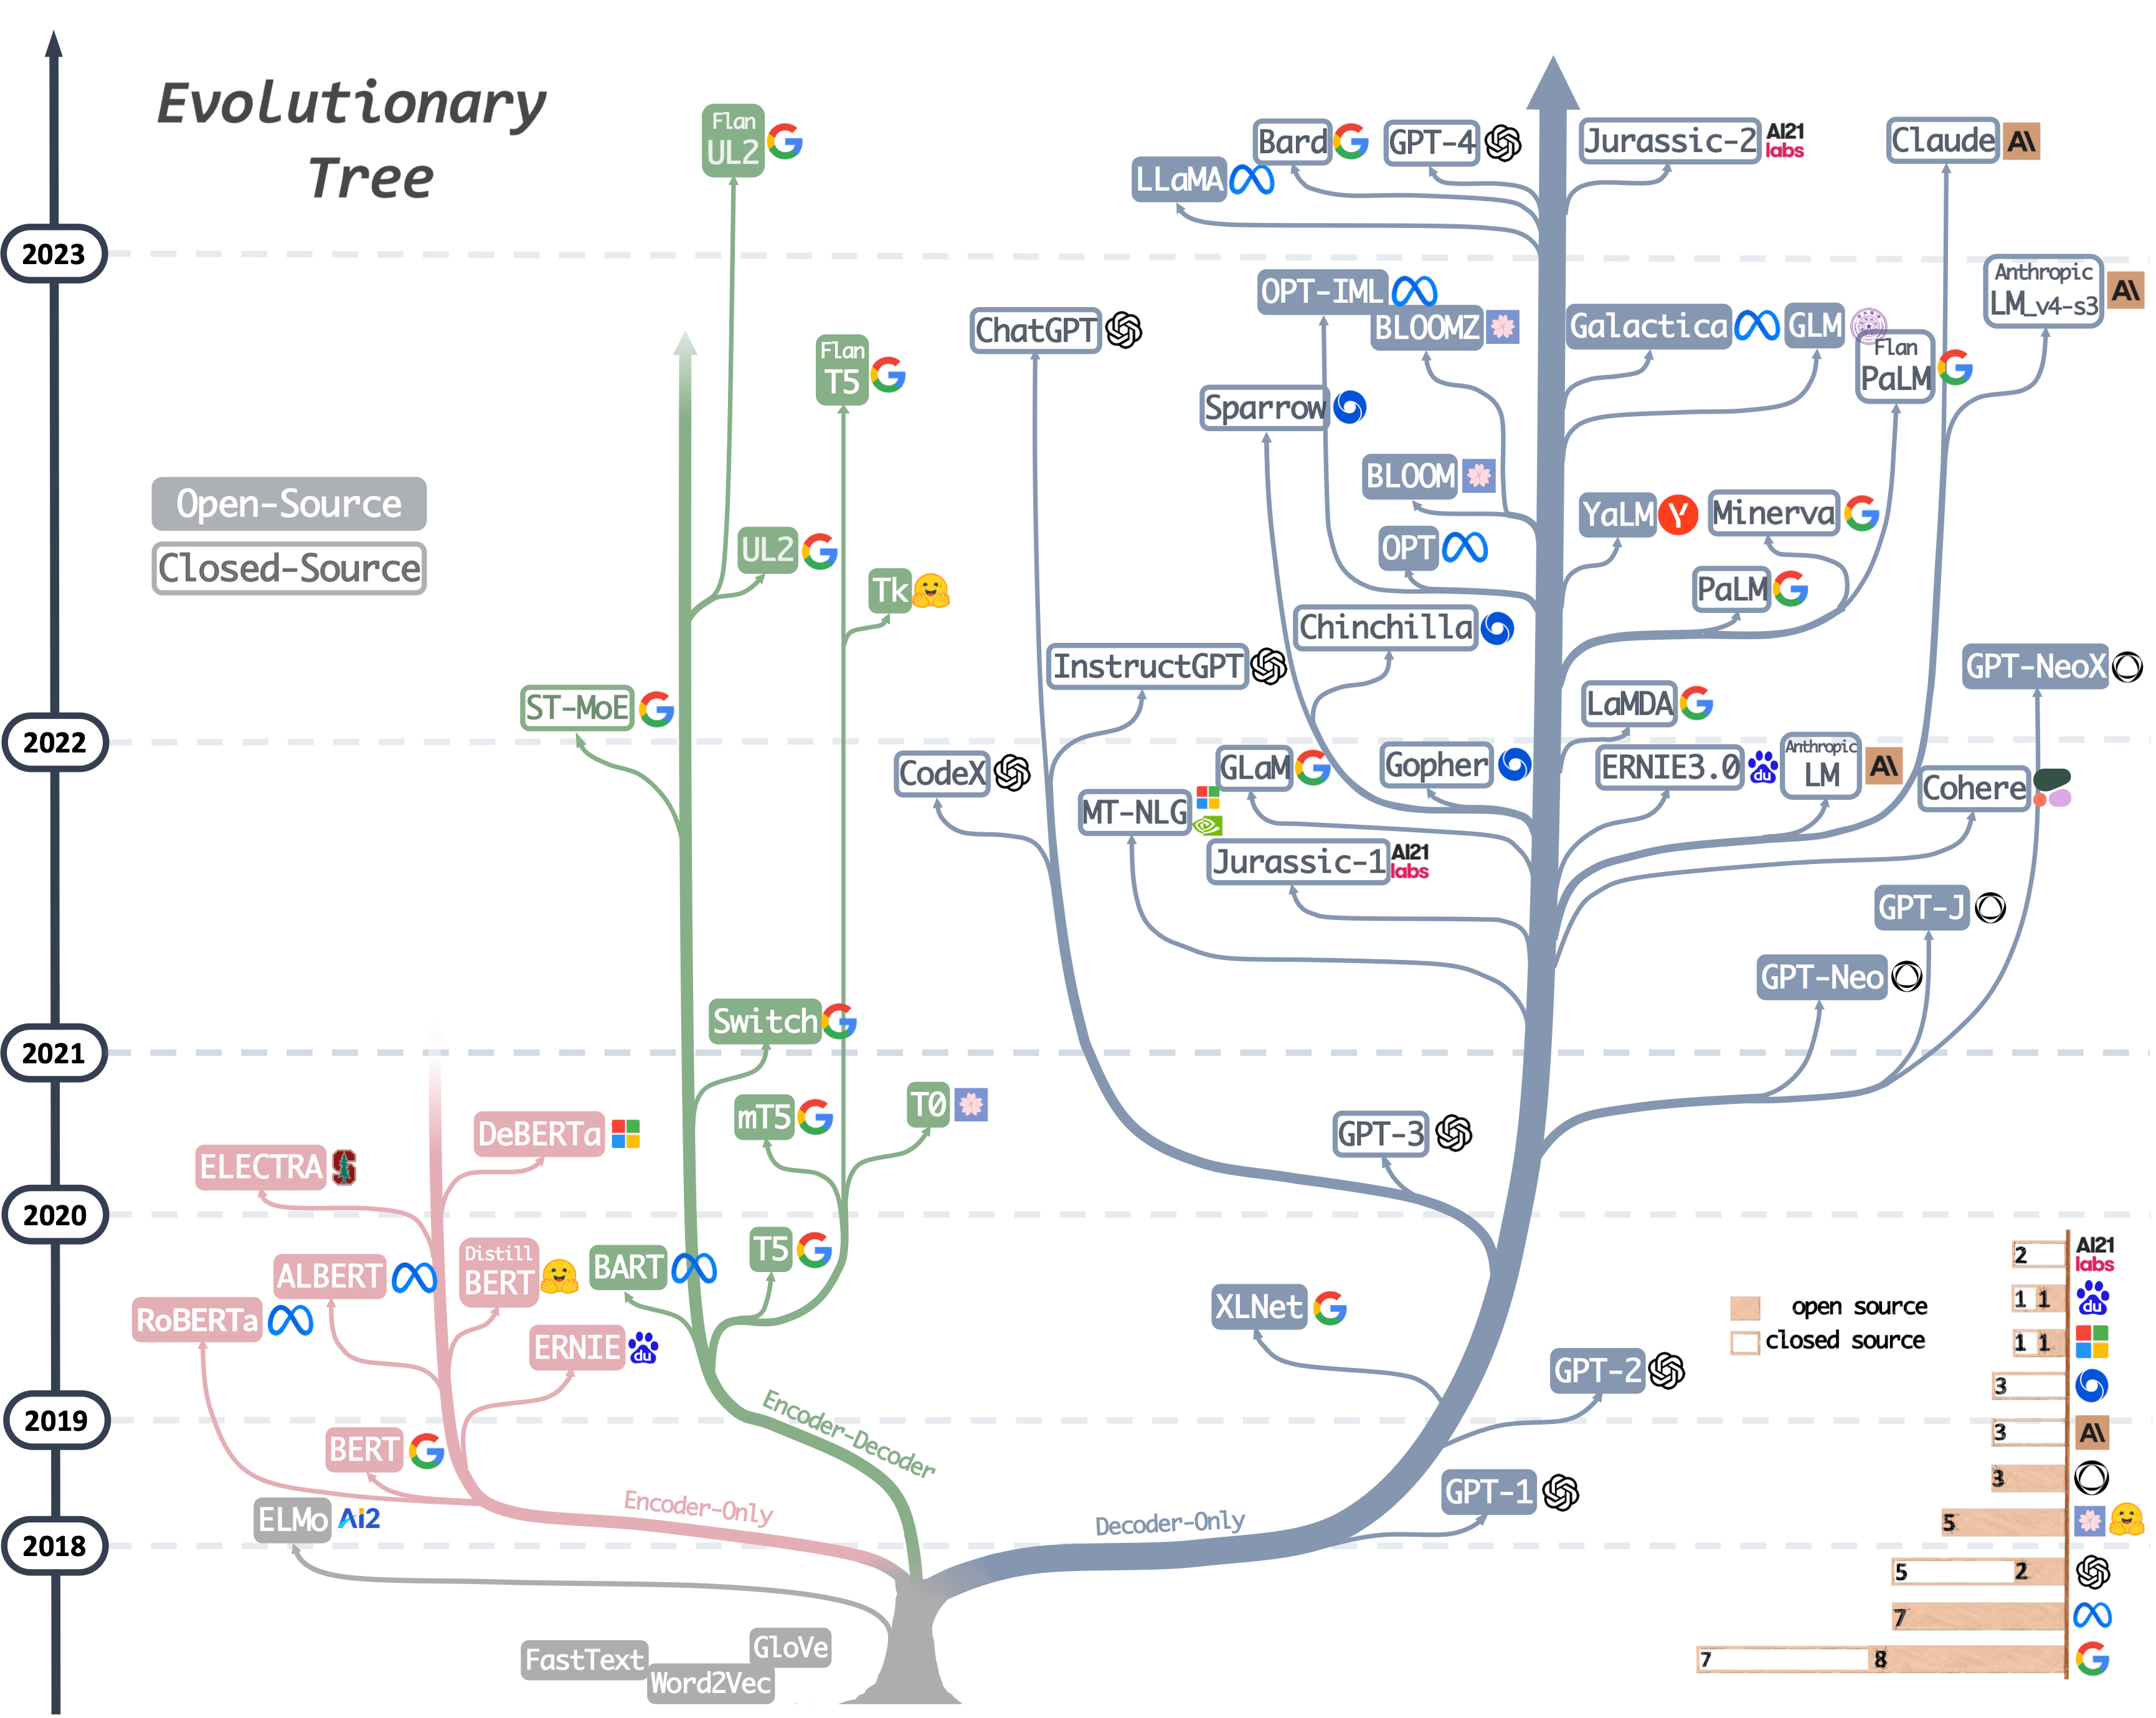
\includegraphics[width=0.7\textwidth]{data/images/tree.png}
  \caption{Übersicht über State-of-the-Art von großsprachigen Sprachmodellen \autocite{yang_harnessing_2023}} \label{fig:stateOfTheArt}
\end{figure}

Mithilfe der \autoref{fig:stateOfTheArt} lässt sich verdeutlichen, dass in dieser Arbeit ausschließlich ältere Methoden werden, verglichen mit Encoder-Decoder und Decoder-Only Modellen. So wurden seit \num{2021} keine neuen Encoder-Only Modelle mehr veröffentlicht, aber im Gegenzug sehr viele Decoder-Only Modelle. Der erste Grund ist, dass viele der neueren, größeren Modelle nicht öffentlich sind und sich daher nicht verwenden lassen. Weiterhin sind viele \ac{NLP} Modelle ausschließlich in englischer Sprache verfügbar, da sie universell ist und bei Weitem mehr Datensätze existieren. Es gibt zwar multilinguale Modelle, jedoch erreichen diese meist nicht so gute Ergebnisse wie sprachspezifische Modelle. Hinzukommt, dass sowohl multilinguale als auch neuere, öffentlich zugängliche, deutsche Modelle deutlich mehr \ac{GDDR5} Speicher benötigen, der im Rahmen dieser Arbeit nicht zur Verfügung steht. Die in dieser Arbeit verwendeten Methoden sind demzufolge nicht State-of-the-Art. Es ist zu erwarten, dass neuere, leistungsstärkere Modelle einen signifikanten Effekt auf die in \autoref{ch:crispDm_2} gemessene Modellperformance haben würden.

\section{Weitere Experimente} \label{subsec:furtherExperiments}

Aus dem \nameref{ch:crispDm_2} und der Diskussion ergeben sich offene Fragen zu Zusammenhängen und Auswirkungen einzelner Entscheidungen in dieser Arbeit. Einige davon sollen im folgenden Abschnitt weiter untersucht werden.

In \autoref{ch:crispDm_2} und anhand der Konfusionmatrizen in \autoref{ch:dataAppendix} zeigt sich, dass die Modelle teils sehr anfällig für unbalancierte Daten sind. Angesichts dessen werden alle weiteren Experimente ausschließlich mit ausbalancierten Trainingsdaten durchgeführt. Die Testdaten bleiben nach wie vor unangetastet.

\subsection{Out-of-domain} \label{subsec:outOfDomain}

Bei jeglicher Form von \ac{ML}-Modellen stellt sich die Frage, wie allgemeingültig das jeweilige Modell angewendet werden kann. Ähnlich zu \textcite{biessmann_predicting_2016} werden zur Überprüfung dessen Modelle verwendet, die lediglich auf einem der drei Datensätze trainiert werden. Anschließend werden alle unbalancierten Datensätze auf Basis des gewählten Modells getestet. Alternativ dazu lässt \textcite[1631]{guhr_training_2020} jeweils einen der Datensätze aus dem Training. Anschließend wird der fehlende Datensatz genutzt, um diesen auf dem trainierten Modell zu testen. Damit lässt sich einerseits die Verbesserung für das gesamte Modell anhand eines Datensatzes nachweisen, als auch die Performance auf neuen Daten feststellen. Schlussendlich wird noch ein Modell auf allen Daten trainiert. Der Zieldatensatz wird jedoch lediglich zu \SI{80}{\percent} für das Training genutzt. Die restlichen \SI{20}{\percent} stellen den Testdatensatz dar.

Das Training wird mit \ft durchgeführt, da es eine geringe Trainingsdauer bei dennoch hoher Genauigkeit hat. Für das Training werden dieselben Parameter wie in \autoref{sec:trainingFastText} verwendet. Als Bewertungsmetrik wird der Makro \(F_{1}\) Score verwendet. \autoref{tab:overviewScoresOutDomain} zeigt die Ergebnisse für die unterschiedlichen Durchläufe und Kombinationen.

{\footnotesize
\begin{longtblr}[caption={Out-of-domain Makro \(F_1\) Score für \ft Modelle}, label={tab:overviewScoresOutDomain}, remark{Anmerkung}={Training und Testing erfolgt jeweils auf den gesamten Datensätzen}, remark{Parameter} = {\(E = \num{20}\), \(LR_{init} = \num{0.1}\)}, note{1}={In-domain (Ergebnisse aus \autoref{sec:trainingFastText})}, note{2}={Zieldatensatz in \SI{80}{\percent} Trainings- und \SI{20}{\percent} Testdaten aufgeteilt}]{width=0.75\textwidth, hline{1, 3, Z} = {0.75pt}, rowhead = 2, colspec={cX*{3}{Q[si={table-format=1.2},c]}}, row{1-2}={guard,font=\bfseries,l}}
     & & \SetCell[c=3]{c} Test & & \\ 
    \cline{3-5}
     & Datensatz & Tweets & Wahlprogramme & Reden \\ 

    \SetCell[r=5]{c} \rotatebox[origin=c]{90}{\textbf{Train}} & Tweets & 0.58\TblrNote{$1$} & 0.36 & 0.44 \\*
     & Wahlprogramm & 0.23 & 0.54\TblrNote{$1$} & 0.25 \\*
     & Reden & 0.22 & 0.31 & 0.65\TblrNote{$1$} \\*
     \cline{2-5}
     & \num{2} von \num{3} & 0.27 & 0.36 & 0.43 \\*
     & Kombiniert\TblrNote{$2$} & 0.56 & 0.49 & 0.68 \\
\end{longtblr}
}

Als Erstes wird die out-of-domain Performance für das Training auf einzelnen Datensätzen evaluiert. In \autoref{tab:overviewScoresOutDomain} zeigt sich, dass die Modelle trainiert auf den Wahlprogrammen und Reden bei der Anwendung auf die jeweils anderen Datensätze mit \numrange{0.22}{0.31} schlechte Ergebnisse liefern. Im Vergleich lässt sich in-domain auf den Datensätzen ein gut doppelt so hoher \(F_1\) Score erreichen. Das Modell ausschließlich auf den Tweets schneidet im Vergleich besser ab. Dieses erreicht \(F_1\) Scores von \numrange{0.36}{0.44} auf den Wahlprogrammen und Reden. Die naheliegendste Ursache für diese Unterschiede ist die Korrelation zwischen der Performance und der Anzahl an Einträgen für das Training. Alternativ, ist es denkbar, dass die Trainingstextsorte einen Einfluss auf die Allgemeingültigkeit eines Modells hat.

Das nächste Experiment deutet ebenfalls auf einen Zusammenhang zwischen der Genauigkeit und der Anzahl an Trainingsdaten hin. Wenn das Modell auf zwei der drei Datensätze trainiert wird, schneiden die Tweets am schlechtesten ab. Die Wahlprogramme erreichen einen \(F_1\) Scores von \num{0.36}, während die Reden mit \num{0.43} das beste Ergebnis erzielen. Das Modell, trainiert auf den Wahlprogrammen und Reden, schneidet besser ab als die vorherigen in-domain Experimente. Die anderen beiden Kombinationen erreichen lediglich gleiche Ergebnisse oder schneiden um \num{0.01} leicht schlechter ab.

Die besten Ergebnisse erzielt mit Abstand das Training auf allen Datensätzen. Damit werden Werte zwischen \numrange{0.49}{0.68} erreicht. Auf den Reden lasst sich sogar ein um \num{0.03} besserer Score verglichen mit der in-domain Variante erreichen.

Zusammenfassend kann gesagt werden, dass \ft in den genannten Konfiguration nur bedingte Fähigkeiten besitzt, um out-of-domain Daten zu klassifizieren. Das Modell schneidet deutlich besser ab, wenn die Zieltextsorte ebenfalls Teil des Trainingsdatensatzes ist.

\subsection{Erweiterter Zeitraum}

Die These, dass eine Eingrenzung des Untersuchungszeitraums für eine gute Performance des Modells notwendig ist, wird im Folgenden untersucht. Dazu wird der Reden-Datensatz genutzt, da dieser bereits alle Reden der vergangenen Wahlperioden geordnet bereithält. Ausgehend von der \num{19}. Wahlperiode wird der Zeitraum, den der Trainingsdatensatz umfasst, schrittweise bist zur \num{16}. Wahlperioden erweitert. Dabei werden jedes Mal zufällig \num{25000} Reden ausgewählt, um durch die unterschiedliche Anzahl an Reden kein Bias zu erzeugen. Für jeden Zeitraum wird einerseits das \ft Modell und andererseits die Lineare \ac{SVC} mit \ac{TF-IDF} trainiert, weil beiden Modelle schnell zu trainieren sind und eine vergleichbar gute Performance in \autoref{ch:crispDm_2} aufweisen.

\begin{table}[H]
    \centering
    \caption{Makro \(F_1\) Score für Reden verschiedener Zeiträume} \label{tab:overviewScoresExtendedPeriod}
    {\footnotesize
    \begin{tblr}{width=\textwidth, hline{1-2, Z} = {0.75pt}, colspec={c*{2}{Q[si={table-format=1.2},c]}}, row{1}={guard,font=\bfseries,l}}
        Wahlperiode(n) & \ft & Lineare SVC \\ 

        \num{19} & \textbf{\num{0.68}} & \textbf{\num{0.66}} \\
        \numrange{18}{19} & 0.65 & 0.61 \\ 
        \numrange{17}{19} & 0.61 & 0.59 \\ 
        \numrange{16}{19} & 0.60 & 0.57 \\ 
    \end{tblr}
    }
\end{table}

\autoref{tab:overviewScoresExtendedPeriod} stellt die \(F_1\) Werte beider Modelle für die vier untersuchten Zeiträume nach Wahlperioden dar. Sowohl für \ft als auch für die Lineare \ac{SVC} erreicht den höchsten Score, wenn ausschließlich der Datensatz der \num{19}. Wahlperiode genutzt wird. Bei jeder Erweiterung um eine zusätzliche Wahlperiode reduziert sich das Ergebnis bei \ft um \numrange{0.01}{0.04} und bei den Linearen \acp{SVC} um \numrange{0.02}{0.05}.

Diese Beobachtungen bestätigen die These, dass Faktoren wie Sprache und Kernthemen zur Abnahme des \(F_1\) Scores führen. Um die These noch weiter zu stützen, müssen ebenfalls die verbleibenden Modelle und mehr Datensätze getestet werden.

\subsection{Daten auf Satz-Ebene}

Um zu überprüfen, welchen Einfluss Daten auf Satz- statt auf Dokument-Ebene haben, werden im Folgenden das \ft und das \ac{CNN}-Modell mit einem modifiziertem Reden- und Wahlprogramm-Datensatz trainiert. Dieser enthält statt ganzen Reden und Absätzen aus Wahlprogrammen alle Sätze als einzelne Einträge. Aufgrund der Länge und nicht eindeutigen Satzstrukturen werden Tweets nicht in Sätze unterteilt. Der kombinierte Datensatz enthält daher nur die Reden und Wahlprogramme, nicht die Tweets.

\begin{table}[H]
    \centering
    \caption{Makro \(F_1\) Score für Sentence-Level Daten} \label{tab:overviewScoresSentenceLevel}
    {\footnotesize
    \begin{tblr}{width=\textwidth, hline{1-2, 4, Z} = {0.75pt}, colspec={c*{2}{Q[si={table-format=1.2},c]}}, row{1}={guard,font=\bfseries,l}}
        Datensatz & \ft & CNN \\ 

        Wahlprogramme & 0.36 & 0.31 \\*
        Reden & 0.31 & 0.27 \\*

        Kombiniert & 0.38 & 0.29 \\
    \end{tblr}
    }
\end{table}

\autoref{tab:overviewScoresSentenceLevel} stellt die Resultate dieses Versuches dar. \ft kommt für die Wahlprogramme auf \num{0.36}, für die Reden auf \num{0.31} und der kombinierte Datensatz erreicht. Die \(F_1\) Scores liegen damit deutlich unter denen des ursprüngliche, Dokumenten-basierten Ansatzes (Wahlprogramme: \num{0.58}; Reden: \num{0.69}). Besonders auffällig ist der Abfall der Performance bei den Reden, deren Genauigkeit um über die Hälfte einbricht. Für den \ac{CNN}-Ansatz reduzieren die alternativen Datensätze die Performance um \num{0.17} für die Wahlprogramme und um \num{0.21} für die Reden.

Durch die Aufteilung in Sätze entsteht ein Vielfaches an Einträgen in den Datensätzen: Die Wahlprogramme wachsen von \num{27674} auf \num{113505}; die Reden von \num{38475} auf \num{603799}. Bei diesem Anstieg kann allerdings nicht gleichzeitig gewahrt werden, dass den \ac{ML}-Modellen ausreichend Kontext und Information für jeden Datensatzeintrag gegeben wird. Folglich kann festgehalten werden, dass die Dokumenten-basierte Herangehensweise für die gewählten Modelle deutlich geeigneter ist als die Satz-basierte.

\section{Bereitstellung eines Klassifikationsmodells} \label{sec:crispDm_4}

Hugging Face ist eine Plattform, die es unter anderem ermöglicht, \ac{ML}-Modelle öffentlich bereitzustellen. Im Rahmen dieser Arbeit wird das auf Basis von \texttt{distilbert-base\--german-cased} trainierte Modell zur Verfügung gestellt. Es handelt sich dabei um die Version, die auf den kombinierten, balancierten Daten trainiert wurde. Dadurch soll vermieden werden, dass das Modell nur eine Textsorte gut erkennt und einen Bias aufgrund der Anzahl an Einträgen pro Partei aufweist. Das Modell wird unter dem Namen felixhoffmnn/GePart\footnote{\href{https://huggingface.co/felixhoffmnn/GePart}{https://huggingface.co/felixhoffmnn/GePart}} auf Hugging Face bereitgestellt und lässt sich auf der Plattform ebenfalls testen. Ebenso wie der Quellcode für diese Arbeit unterliegt das Modell der GNU General Public License v3.0.

\textbf{Disclaimer:} Die Gesamtleistung (gemessen am \(F_1\) Score) mit \num{0.58} ist verbesserungswürdig, sodass fehlerhafte Klassifikationen zu erwarten sind. Zusätzlich dazu weist das Modell Biases durch die Wahl der Textsorten, dem Untersuchungszeitraum und den politischen Themen auf. Daher sollten die Ergebnisse, die das Modell liefert, mit äußerster Vorsicht betrachtet werden. Außerdem wird keine Haftung für unethische Klassifikationen übernommen.
